\chapter{Background}\
\label{chap:background}
This section tackles the fundamental principles and groundwork of the theory encompassing concepts, terminology, and methodologies related to search engines as applied within this thesis. Section \ref{sec:web-search-engine} dives into the essential components and characteristics required to implement the search engine discussed in this thesis. Section \ref{sec:crawler} provides a comprehensive examination of the crawler's specifications and architecture. Section \ref{sec:indexing} offers an in-depth explanation of the fundamental indexing terms and concepts essential to this thesis, while Section \ref{sec:ranking} explores the ranking score used in this research.


\section{Web Search Engine}
\label{sec:web-search-engine}
Web Search Engine is software that collects information from the web and indexes them efficiently to optimize the searching process by the end user. When users enter their queries to ask for information, the engine performs queries, looks up the pre-built organized index, and returns relevant results. Search Engine Results Pages, known as SERPs, present the returned results. The result is then ranked based on predefined criteria. 

Web search engines use web crawlers or spiders to collect and harvest the internet, jumping from one page to another. Each page can contain several links. The crawler's task is to find the links, visit them, and harvest them. Followed by crawlers, indexing is the next process where information is organized and optimized for search.

\begin{figure}[h]	
     \centering
         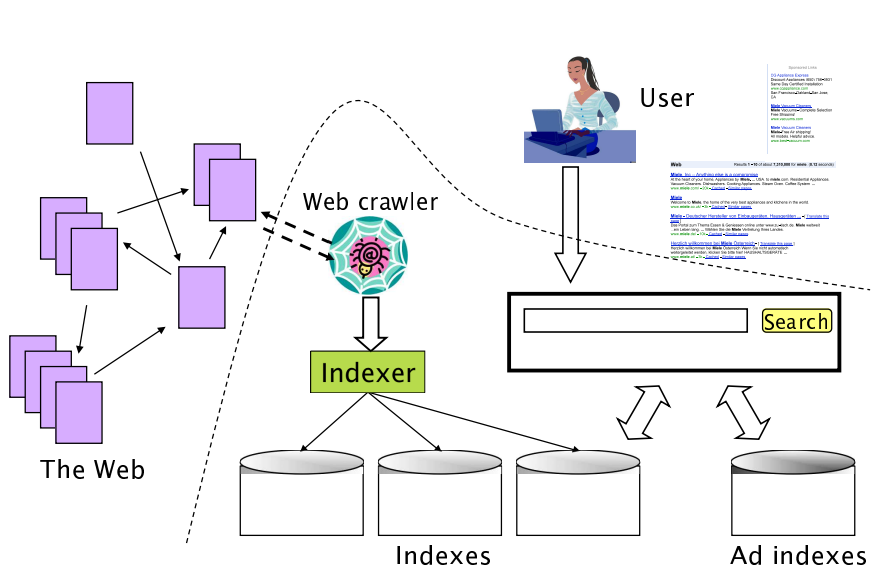
\includegraphics[width=10cm]{images/engine_components.png}
              \caption{An overview of a generic search engine system.}
     \label{fig:search-engine-overvoew}
\end{figure}

\subsection{Requierments and Features}
Regardless of their implementation and design, all search engines share certain features and prerequisites crucial for their effectiveness. Below is a compilation of the most essential features: 

\begin{itemize}
	\item[] \textbf{Web Crawling and Indexing:} As shown in Figure \ref{fig:search-engine-overvoew}, the initial step in the search engine's operation is web crawling. Crawlers initiate the process by connecting to the web and downloading the required pages. Subsequently, indexing comes into play, where the downloaded files are organized and indexed to enhance querying and search efficiency. Parsing the downloaded pages can be carried out in either the crawling phase or during indexing, and Scriburg, this parsing occurs during the crawling process. It is worth noting that, in Scriburg, pages are not downloaded; the targeted documents are parsed, stored in the database, and the pages themselves are discarded.
  \item[] \textbf{Ranking and Relevancy:} As indicated in Figure \ref{fig:search-engine-overview}, when users input a query to search for relevant documents, they face the Search Engine Results Pages (SERP). Users typically focus on the top results while overlooking the lower results. Hence, we must maintain relevancy. Ensuring relevance is a challenging task. Ranking the discovered documents and prioritizing the most pertinent documents at the top and the less relevant ones further down is crucial. 
  \item[] \textbf{Scalability and Performance:} A distributed system is essential for managing the extensive data and traffic demands. A load balancer is critical in distributing the crawling tasks efficiently among nodes and threads. In this, we will discuss the implemented loading balance mechanism to distribute the crawling tasks among the crawlers. 

\end{itemize}

\section{Cralwer}
\label{sec:crawler}
Web crawler or spider is a software which gathers pages information from the web, to prived the necessary data to the Indexer to build a search engine. The essential role of crawlers is to effectively and reliably collect as much information from the web as possible. This thesis invests more time on this component than the Indexer as it serves as the bottleneck to the Search engine performance. 

\subsection{Cralwer Specifications}
Crawlers can display a diverse range of features and specifications. Nevertheless, certain essential elements must be incorporated, while others are critical for ensuring a reliable and functional crawler. Further details can be explored in the book referenced as \cite{introduction-ir}.

\begin{itemize}
\item[] \textbf{Robustness:} Web crawlers can be fragile and easy to break due to the nature of the dynamic contents on the web and the internet connection. Web crawlers must identify those edge cases and obstacles and tackle them.   

\item[] \textbf{Politeness:} The crawler implementation can be unintentionally dangerous if incorrectly designed. A Denial of service DoS and a Distributed Denial of service DDoS attacks can occur due to an irresponsible crawler implementation. Hence, crawlers must respect website policies and avoid breaking up web services and loading the servers.

\item[] \textbf{Performance and Efficiency:} The crawling system should use various resources, such as processing power, storage capacity, and network bandwidth. Moreover, the crawler should be able to function in distributed microservices across multiple machines.

\item[] \textbf{Freshness:} Obtaining recent versions of previously accessed pages, ensuring the search index remains updated.
\end{itemize}

\subsection{Crawler Architecture}

The simple crawler architecture is made of the following fundamental modules, as shown in the following Figure. Fetch module that communicates with the internet and collects the pages passed by the URL Frontier module using HTTP requests from the URLs. URL frontier module contains a list of the URLs that need to be fetched by the Fetch module. Parsing module that takes the page content found by the fetch module and parses the page content to find the following links to be passed to the URL frontier and also to parse any value needed from the page, like text and images. Duplication filter that is used to exclude seen URLs. The DNS resolution module is responsible for identifying the web server from which to retrieve the page indicated by a given URL [9]. 

\begin{figure}[h]	
     \centering
     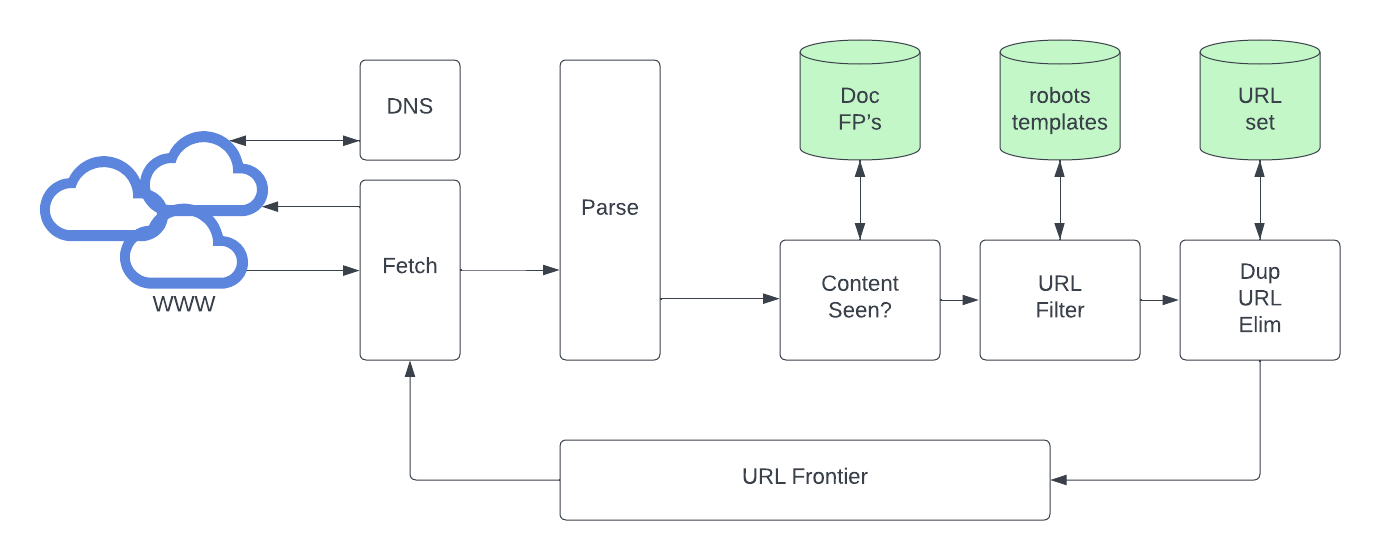
\includegraphics[width=10cm]{images/crawler_architecture.png}
     \caption{The basic crawler architecture.}
     \label{fig:google-arch}
\end{figure}

The first step is to add a seed URL to the URL frontier. This URL works as a starting point for crawling. The crawler then fetches the page corresponding to the seed URL and stores it to be parsed by the parser. Subsequently, the page undergoes parsing to extract both its textual content and embedded links. The content will be used by the indexer component in the search engine. Moreover, each identified link by the parser module is subjected to a set of evaluations to determine its eligibility for addition to the URL frontier.

After finding the future links and content by the parser, filtering both found links and content is needed. The first step is to check if the page content has already been seen; this can be done by checking the page content fingerprint. The most straightforward method is to use a checksum (stored in the Doc FP's). The next filter is to exclude the parsed new URLs. The URL filter will run some tests to exclude unwanted URLs. This can be some URLs out of the country target, like .de, or some restricted URLs that should not be visited by the crawler. Excluded URLs list can be added manually to the filter. However, there are more rules written by the domain admins that should be followed. Those rules can be found under a standard text file named Robots Exclusion Protocol (robots.txt). 

"robots.txt" acts as the selected filename for implementing the Robots Exclusion Protocol, which is a widely adopted standard employed by websites to signal to web crawlers and other web robots the specific sections of the website that are permissible for them to access [10]. The "robots.txt" can be fetched at the starting point of crawling and can be cached through the whole crawling process, as it can be assumed it will not change during the crawling process. This assumption is still better than making an HTTP request to get the robots.txt file for each URL that needs to be fetched, as this will duplicate the number of requests and reduce the crawler efficiency and also load the server with unwanted requests. Including the robots.txt in the crawling, process should be mandatory as this will serve the point about politeness mentioned in the Crawler specifications section. 

\subsection{Web Crawler Types}
It is essential to understand that although all web crawlers' main goal is to crawl pages from the internet, however, there are different types and categories that some crawlers fall to. The first category is  \textbf{Universal or Broad crawler}. This category of web crawlers doesn't confine itself to webpages of a specific topic or domain; instead, they continuously traverse links without limitations, collecting all encountered webpages. The most significant search engines use this type of crawler, such as Google and Bing, this is understandable as these search engines' main aim is to make the entire web searchable, and they try to fetch all kinds of pages and contents. The second category is called \textbf{Preferential crawler (Focused crawler)}. Focused crawlers target specific topics, themes, or domains. They are designed to gather information from a particular niche or subject area, providing specialized search results. In this thesis, a Focused crawler has been implemented and used. The last category is \textbf{Hidden Web crawlers (Deep Web Crawlers)}. Deep web crawlers target databases and content hidden behind web forms. They can interact with online databases and retrieve information that general search engines might miss [11].

\subsection{Challenges and issues}
Researchers encounter a variety of challenges when working with different crawlers implementation. A compilation of these challenges is presented below.


\begin{itemize}
\item The scale of the web: The web is vast and virtually infinite, so crawlers must prioritize which pages to crawl and which to skip to use resources efficiently.

\item Content Changes: Webpages can change frequently, requiring crawlers to revisit and reindex content to ensure freshness and accuracy.

\item Blocking and IP Bans: Some websites may block or ban crawlers' IP addresses if they perceive them as causing too much traffic or disruption. Crawlers need to manage IP addresses to avoid being blocked.

\item Nonuniform structures: The Web is dynamic
and uses inconsistent data structures, as there is
no universal norm to build a website. Due to lack of uniformity, collecting data becomes difficult. The problem is amplified when crawler has to deal with semistructured and unstructured data.

\item Error handling: Crawlers may encounter broken links, leading to errors and incomplete indexing. Handling broken links requires additional processing. Moreover, the internet connection may disconnect, and the crawler may stop crawling. 

\item Crawlers traps: Some websites intentionally create spider/crawlers traps to make crawlers go into an infinite loop or redirect them in different directions. Calendar Traps and Infinite URL Parameters are examples of spider traps.

\item Politeness and Ethical Concerns: Crawlers must be programmed to be polite and respectful to websites' server resources. Aggressive crawling can overload servers, leading to ethical concerns and potential website blocking. This might be simple, but the main challenge is that each domain uses different Firewall settings. One server might allow the crawler to make five requests per second; the other will block the crawler. There are no hardcoded rules to follow; however, following the robots.txt file might help improve the  Politeness of the crawler.
\end{itemize}


\\


\section{Indexing}
\label{sec:indexing}
In a search engine, an indexer is a component responsible for analyzing and organizing the content of web pages or documents in order to create an index, which is a structured database that enables efficient and fast retrieval of relevant information during search queries.
When a search engine's crawler or web spider gathers data from websites, the indexer processes this data by breaking down the content into smaller units like words, phrases, and metadata. It then associates these units with the URLs or documents they came from. This organized information is stored in the index, which serves as a map or reference for the search engine to quickly locate and present relevant results when a user makes a search query.
The indexer plays a crucial role in improving the speed and accuracy of search results because it precomputes and structures the data in a way that enables the search engine to match queries with indexed content more efficiently. Although supporintg indexing is fundemantal in this thesis however it will be given less attention than the crawling component. 

\subsection{Inverted index}
Crawlers collect information from the web and prepare them to be searched. However, looking up each term with brute forcing is a performance issue and is impossible. Hence inverted index data structure is used. 
An inverted index or inverted file is a data structure used in information retrieval systems, particularly in search engines, to store and efficiently retrieve information about the occurrences of terms (words or phrases) within a collection of documents. It is called "inverted" because it inverts the relationship between terms and documents compared to traditional databases, where documents are associated with their content.
In an inverted index, each unique term in the collection of documents is treated as a key, and the value associated with each term is a list of references to the documents where that term appears. This list of references allows for rapid access to all the documents containing a specific term.

Creating an Inverted index requires the next steps. The first step is to collect the documents to be indexed. In the context of this thesis, the documents referred to the content inside the crawled pages. The second step is to tokenize the text, turning each document into a list of words known as tokens. The last step is to create a dictionary that maps each term with a list of the ids of the documents that occurred. The tokenized terms are called dictionaries, and the list of ids is called postings. 

\begin{figure}[h]	
     \centering
     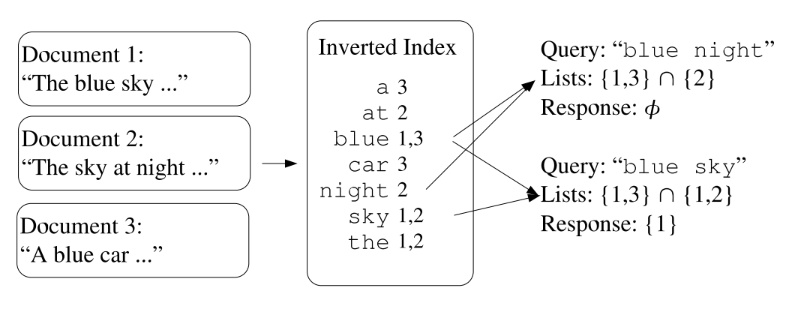
\includegraphics[width=10cm]{images/inverted_index.png}
     \caption{
An illustration of an inverted index featuring three documents. All tokens are included in this example, and the sole text normalization applied is converting all tokens to lowercase. Queries that involve multiple keywords are resolved using set operations. [3]}
     \label{fig:google-arch}
\end{figure}

\subsection{Document Unit}
The term "document" has frequently been mentioned in reference to the specific information intended for retrieval from a webpage. While, in most instances, this term encompasses the entirety of a page's content, this holds true primarily for Universal crawlers. However, in the case of the Preferential crawler employed in this thesis, the definition of a document unit is adaptable, contingent upon the nature of the website and the specific data the user seeks to gather. For instance, in an E-commerce website featuring product titles, prices, and descriptions, the document unit may be viewed as a single product listing. Conversely, a news website might treat each news article as an individual document. More comprehensive guidance on creating a template that corresponds to a document will be provided in the Approach chapter.

\subsection{Tokenization}
Tokenization in indexing is the process of breaking down a text document or a string of text into smaller units called tokens. These tokens are typically words or subwords, and they serve as the basic units for indexing and searching within a text corpus. Tokenization is a fundamental step in natural language processing and information retrieval tasks.

\fbox{\begin{minipage}{15em}
Input: The University of Freiburg
Output: The University of Freiburg
\end{minipage}}

\section{Ranking}
\label{sec:ranking}
As discussed indexing process prepares a map that can be looked up to find relevant terms that match the search query; however, one needs to rank the returned result based on relevance. For example, a user searching "for what is Freiburg?" will be expecting a result about Freiburg and not to return all documents that contain tokens like "what" and "is". So how can we find the relevant documents? There are many algorithms for document ranking. However, in this thesis, BM25 will be adopted. 

\begin{equation}
BM25\_score = tf^*.\log_2(\frac{N}{df})
\label{eq:depth}
\end{equation}
\begin{equation}
tf^* = \frac{tf.(k+1)}{k.\alpha+tf}
\label{eq:depth}
\end{equation}
\begin{equation}
\alpha = \frac{1-b+b.DL}{AVDL}
\label{eq:depth}
\end{equation}

\textit{N} = Total number of docuemnts, \textit{tf} = term frequency, the number of times a word occurs in a document, \textit{df} = docuemnt frequency, The number of documents containing a particular word, \textit{DL} = document length, \textit{AVDL} =
average document length (measured in number of words)
Standard setting for BM25: \textit{k} = 1.75 and \textit{b} = 0.75.

The following example dives into the details of the BM25 equation and how it impacts ranking.  Table [] shows a list of documents as an example of an input to be indexed and ranked against different search queries. We start by calculating the variables needed to find the BM25 scores for each term in a document.    

Since we have three documents, the N variable will equal 3. The second step is to find document length DF for each document {1: 26, 2: 21, 3: 49}. AVDL will equal 32. Plugging those values into the equation, we get an inverted list as follows: 

\begin{table}[ht] 
{\footnotesize
\begin{tabular}{ P{2.5cm} ||P{11.1cm}  }      % centered columns (3 columns) 
 \hline \hline
Document ID & Document content\T\B 
\\ 
\hline
1 & The University of Freiburg, officially the Albert Ludwig University of Freiburg, is a public research university located in Freiburg im Breisgau, Baden-Württemberg, Germany.\T\B 
\\ 
\hline
2 & Freiburg im Breisgau, usually called simply Freiburg, is an independent city in the state of Baden-Württemberg in Germany.\T\B 
\\ 
\hline
3 & A university from Latin universitas 'a whole' is an institution of higher (or tertiary) education and research which awards academic degrees in several academic disciplines. Universities typically offer both undergraduate and postgraduate programs. In the United States, the designation is reserved for colleges that have a graduate school.\T\B 
\\ 
\hline \hline
    \end{tabular}
}
  \captionsetup{justification=centering,margin=2cm}
  \caption{Documents sample}
\end{table}

Examining Table [], we can note that the tokens that appear in all three documents, like 'the', 'of' and 'is' have scores of 0. If the term searched for is common, we should give less weight or value to the search query. For example, users often search for queries such as 'What is ...', 'who is ..' , and 'Where is ...'. Those queries contain common words that are not informative in documents like 'What', 'Who', 'Where' and 'is', the term coming after those sentences should be more valuable and have more weight. Unique words like 'albert' and 'ludwig' have high scores as they only occur in one document. Words like 'freiburg' and 'university' have different scores for each document depending on the word's appearance relative to the document's length. 

\begin{table}[ht] 
{\footnotesize
\begin{tabular}{ P{2.5cm} ||P{11.1cm}  }      % centered columns (3 columns) 
 \hline \hline
Token & (Doc. ID, BM25 Score)\T\B 
\\ 
\hline
the & [(1, 0.0), (2, 0.0), (3, 0.0)] \T\B 
\\ 
\hline
university &  [(1, 1.071), (3, 0.466)] \T\B 
\\ 
\hline
of  &  [(1, 0.0), (2, 0.0), (3, 0.0)] \T\B 
\\
\hline
freiburg  &  [(1, 1.071), (2, 0.975)] \T\B 
\\ 
\hline
officially  &  [(1, 1.740)] \T\B 
\\ 
\hline
albert  & [(1, 1.740)]\T\B 
\\ 
\hline
ludwig  &  [(1, 1.740)] \T\B 
\\ 
\hline
is  & [(1, 0.0), (2, 0.0), (3, 0.0)] \T\B 
\\ 
\hline
a  & [(1, 0.642), (3, 0.885)] \T\B 
\\ 
\hline
public  &  [(1, 1.740)] \T\B 
\\ 
\hline \hline
    \end{tabular}
}
  \captionsetup{justification=centering,margin=2cm}
  \caption{The first 10 tokens of the result inverted index and the scores of the docuemnts. }
\end{table}

User search for 'university of freiburg' will return the next result: (1, 2.14), (2, 0.97), (0.46). The first document with id 1 has the highest score as it contains both words. This is the correct result, as the first document talks about the university of freiburg. The second document 2, which talks about the city Freiburg, is higher than the third because freiburg is mentioned twice in the same document, and the content is shorter. The next section will examplin how can one refine the ranking of documents.

\subsection{Ranking Refinements}
Some methods can be implemented to boost the document's ranking. The first step is to focus on tokenization of the documents. 

In the previous example, we can note that the univerisy term has appeared in documnet 3 only once; however, the term universities appeared twice. In the ranking, the relation between the two words is not achieved because the inverted index will include university and universities separately. This will reduce the score of document 3 when the user searches for university, although both terms are associated and linked and should be accumulated. Stemming and lemmatization, Both stemming and lemmatization aim to simplify inflectional forms and occasionally derivationally related forms of a word, bringing them down to a shared foundational form. As an example:

am, are, is ⇒ be \\
car, cars, car’s, cars’ ⇒ car

Stemming typically involves employing a simple rule-based approach to truncate word endings, aiming to achieve accurate results in most cases. This approach often involves eliminating derivational affixes. In contrast, lemmatization follows a more meticulous process that involves utilizing vocabulary and morphological analysis of words. The primary objective is to exclusively remove inflectional endings and to restore words to their fundamental or dictionary forms, which are referred to as lemmas [5].

We observed that small or frequently occurring tokens such as 'the' and 'of' possess scores of 0, contributing no significance to the overall outcome of the query. Eliminating these terms via stop words can lead to the exclusion of certain frequently used words from the indexing process. A stop words list is a list that holds words that can be excluded from the indexing process. The selection of stop words is language-dependent; each language has its own set of prevalent words. For instance, in English, the subsequent list provides an example of such stop words that could be omitted from the indexing procedure:

a an and are as at be by for from
has he in is it its of on that the
to was were will with


\subsection{Fuzzy search}
As previously explained, the generated inverted index will contain a list of the tokens found on each document, and to find the most relevant document to the user query would be simply to split the query into tokens and search for each token and find its exact matching in the inverted index, then rank the results based on the BM25 scores. Assuming that users will not make any misspelling errors is a hard assumption, especially for some English words; there are differences between British and American spelling, for example, 'color' and 'colour'. Both have the exact same meaning with a different spelling. It would be bad not to return any result if the user chose one word over the other. Other scenarios can also be that the user is not sure about the spelling. For example, 'Freiburg' can be written as 'Frieburg'.  

Fuzzy search is a technique used in natural language processing (NLP) and information retrieval to find approximate matches for a given query or search term, even when the exact spelling or wording might not be present in the target text. This is particularly useful when dealing with typos, misspellings, variations in phrasing, or other types of small deviations from the original text.

Fuzzy search algorithms typically involve techniques like Levenshtein distance (edit distance), which calculates the minimum number of single-character edits (insertions, deletions, substitutions) required to change one string into another. Other techniques include using phonetic algorithms to find similar-sounding words, or tokenization and comparison of word n-grams to identify overlapping substrings.

Considering two character strings, s1 and s2, the edit distance that separates them represents the minimal count of edit operations needed to transform s1 into s2. The typical edit operations permitted for this purpose encompass: (i) the insertion of a character into a string, (ii) the deletion of a character from a string, and (iii) the replacement of a character within a string by another character. In the context of these operations, the term "Levenshtein distance" is sometimes used interchangeably with edit distance. To illustrate, the edit distance between "cat" and "dog" is 3. It's worth noting that the concept of edit distance can be extended to encompass varying weights assigned to different types of edit operations. For instance, assigning a greater weight to the replacement of the character "s" with "p" compared to its replacement with "a" (with the latter being physically closer on the keyboard) can be explored. This weight assignment strategy, dependent on the probability of letter substitutions, proves highly effective in practical scenarios. Nonetheless, the subsequent discussion primarily concentrates on scenarios where all edit operations bear identical weights [5].

Fuzzy search can be used with q-gram to find how similar words are.  For a string x, and an integer q ∈ N, the multiset of q-grams, denoted by Q q(x), , consists of all substrings of length q 3("freiburg") = { "fre", "rei", "eib", "ibu", "bur", "urg" }
We define it as a multiset because the same q-gram may occur multiple times and we want to know when it does 

Q 3("ababa") = { "aba", "bab", "aba" }

The number of q-grams of a string x is:

|Q q(x)| = |x| - q + 1

Similar words have many q-grams in common, that's why it can be used to find similar words. 
Lemma: for strings x and y: |Q q(x) \ Q q(y)| ≤ q ∙ ED(x, y)
Understand: A \ B denotes the set difference, that is, the elements of A without the elements from B If B is very similar to A, then A \ B is small [13]
Example:
x = freiburgerin, y = breifurgerin, ED(x, y) = Q 2(x) = { fr, re, ei, ib, bu, ur, rg, ge, er, ri, in } Q 2(y) = { br, re, ei, if, fu, ur, rg, ge, er, ri, in } 
Q 2(x) \ Q 2(y) = {fr, ib, bu}
|Q 2(x) \ Q 2(y)| = 3

To implement fuzzy search with q-gram, one can use Q-gram index. For each q-gram of a string from D, store an inverted list of all strings from D containing it, sorted lexicographically

\$fr : frankfurt, freiburg, freetown, fresno, …

More information about the implementation will be discussed in the approach section.


\section{The nature of the web}
The web we know today, Web 2.0, is known as "the participative social web" and is massive, and its rate of change is enormous due to its highly dynamic content. Due to this big sample space, finding the relevant pages or documents from the web isn't easy. To overcome this issue, there are two main approaches to sampling: 
Vertical sampling: Focus only on the pages that are restricted by the domain name. This can be done in different levels. For example, one can restrict the crawling process based on the country, such as .de, .ly, uk. When vertical sampling is done at the second level, it limits the crawling to domains (e.g. stanford.edu) [3].
Horizontal sampling: In this approach, it is important to know the most visited pages and domains to keep crawling from them, giving them more priority than others. This can be done by collecting data logs from the ISP or utilising a web crawler to estimate the page's popularity [3]. 


\section{History}
\numberwithin{equation}{chapter}

The World Wide Web is an unlimited space to share provide and share information. Those information can have different format and cover different doamins. The use case of the web is only limtied by the developers imagination. This is benifital as the Web keept evolving rapidaly form Web 1.0 to Web 2.0 to Web 3.0. Web 1.0 used static pages to serve information, those information were moslty news, blogs and personal langing pages. Some refre to the Web 1.0 as "the read-only web". Although Web 1.0 was massive however most content were created was by deverlopers or at least users who knew basics of the HTML and CSS, moreover by that time content were only static they did not depen on fancy JavaScript libraries and frameworks like Angular and React, this made it limited to some use cases only. Fast forward, pages become more dynamic after using sessions, databases and clint rendering schemas. Those changes made the Web focused not only reading and gathering information by gave the power to more audiounce who did not know any programming or coding to participate and interact with the Web via browsers. Social media, e-commerce and trading stocks platforms was one of the reasons made the internet buble inflate, Use cases where unlimited as useres could create and deploy their own websites by using simple tools as Content Manament System CMS. This made Web 2.0 known as "the participative social web".

To optimize the allocation of crawler resources, estimating the page's freshness must be considered. This prevents outdated pages from remaining unrefreshed for prolonged periods or where lesser-significant pages are needlessly recrawled despite unchanged content.


It can be understood intuitively that the likelihood of a copy of page p being up-to-date at time t, denoted as up(t), declines over time when the page is not revisited.

\begin{equation}
u_p(t) \propto e^{-\lambda_pt}
\label{eq:depth}
\end{equation}

The parameter λp signifies the rate of modifications occurring on page p, and its estimation can be deduced from past observations, mainly when the web server indicates the page's last modification date during visits. Cho and Garcia-Molina derived this estimation technique for λp [8].

\begin{equation}
\lambda_p \approx \frac{(X_p-1) - \frac{X_p}{N_p\log(1-X_p/N_p)}}{S_pT}
\label{eq:depth}
\end{equation}

\begin{itemize}
  \item Np number of visits to p.  
  \item Sp time since the first visit to p.
\item Xp number of times the server has informed that the page has changed.
\item Tp total time with no modification, according to the server, summed over all the visits.
\end{itemize}

Note that some pages do not include the last-modified time stamp, and in this case, one can estimate this manually by comparing the
downloaded copies at two different times and using the following equation. Where Xp now will be the number of times a modification is detected.

\begin{equation}
\lambda_p \approx \frac{-N_p\log(1-X_p/N_p)}{S_p}
\label{eq:depth}
\end{equation}
